% tBPSguide.tex
% v2.1 released November 2014

\documentclass{tBPS2e}

\usepackage{epstopdf}% To incorporate .eps illustrations using PDFLaTeX, etc.
\usepackage{subfigure}% Support for small, `sub' figures and tables
\usepackage{lmodern}
\usepackage{color}


\theoremstyle{plain}
\newtheorem{theorem}{Theorem}[section]
\newtheorem{lemma}[theorem]{Lemma}
\newtheorem{corollary}[theorem]{Corollary}
\newtheorem{proposition}[theorem]{Proposition}

\theoremstyle{definition}
\newtheorem{definition}{Definition}

\theoremstyle{remark}
\newtheorem{remark}{Remark}

\begin{document}

%\jvol{00} \jnum{00} \jyear{2014} \jmonth{November}

\articletype{Research Article}

\title{\textit{Simplified Calibration of Urban and Building Multiscale Co-Simulation}}

\author{Clayton Miller\textsuperscript{a}%
$^{\ast}$\thanks{$^\ast$Corresponding author. Email: miller.clayton@arch.ethz.ch}, 
Daren Thomas\textsuperscript{a},
J\'er\^ome K\"ampf\textsuperscript{b},
and Arno Schlueter\textsuperscript{a}\\
\vspace{6pt}
\textsuperscript{a}{\em Architecture and Building Systems (A/S), Institute of Technology in Architecture (ITA), ETH Z\"urich, Z\"urich, Switzerland};\\
\textsuperscript{b}{\em Solar Energy and Building Physics Laboratory (LESO-PB), Ecole Polytechnique F\'ed\'erale de Lausanne (EPFL), Lausanne, Switzerland}
\received{v0.1 released January 2015}
}

\maketitle

\begin{abstract}
This paper describes the simplified calibration process of the building and urban scale models of a campus of higher education buildings. The campus is modeled at both the building scale using the EnergyPlus simulation engine and at the urban scale using the CitySim engine. A co-simulation framework is used to execute simulations from both engines concurrently with an exchange of various information to leverage the various strengths of each. On-site weather and measured performance data is then compared to the output from three modeling scenarios: building-scale simulation, urban-scale simulation, and co-simulation of the engines. A partial calibration process is implemented to reconcile the simulations with the measured data of three targeted buildings. The results illustrate that {\color{red}insert results here}. A discussion is included of the challenges encountered with the urban scale calibration and the strengths and weaknesses of the developed process.
\end{abstract}

%Taken out of the abstract: A significant amount of model input information was extracted for the creation of both models from a building information model (BIM) of the campus.

\begin{keywords}
Building-scale simulation, Calibrated energy models, CitySim, Co-simulation, EnergyPlus, Urban-scale simulation 
\end{keywords}


% {\abstractfont\centerline{\bfseries Index to information contained in this guide}\vspace{12pt}
% \hbox to \textwidth{\hsize\textwidth\vbox{\hsize19pc
% \hspace*{-12pt} {1.}    Introduction\\
% \hspace*{7pt} {1.1.}  The \textit{tBPS} document class\\
% \hspace*{7pt} {1.2.}  Submission of \LaTeX\ articles\\
% \hspace*{24pt}        to the journal\\
% {2.}    Using the \textit{tBPS} class file\\
% {3.}    Additional features\\
% \hspace*{10pt}{3.1.}  Title, authors' names, abstract \\
% \hspace*{24pt}        and keywords\\
% \hspace*{10pt}{3.2.}  Additional footnotes to the title \\
% \hspace*{24pt}        or authors' names\\
% \hspace*{10pt}{3.3.}  Lists\\
% {4.}    Some guidelines for using standard\\
% \hspace*{6pt}         features\\
% \hspace*{10pt}{4.1.}   Sections\\
% \hspace*{10pt}{4.2.}   Illustrations (figures)\\
% \hspace*{10pt}{4.3.}   Tables\\
% \hspace*{10pt}{4.4.}   Landscape pages\\
% \hspace*{10pt}{4.5.}   Theorem-like environments\\
% \noindent \hspace*{7pt} {4.6.}   Typesetting mathematics\\
% \hspace*{24pt} {4.6.1.}   Displayed mathematics\\
% \hspace*{24pt} {4.6.2.}   Bold math italic symbols\\
% \hspace*{24pt} {4.6.3.}   Bold Greek\\
% \hspace*{24pt} {4.6.4.}   Upright Greek characters  \\
% \hspace*{50pt}            and the upright partial \\
% \hspace*{50pt}            derivative sign  \\}
% \hspace{-24pt}\vbox{\noindent\hsize19pc
% \hspace*{7pt} {4.7.}   Acknowledgements \\
% \hspace*{7pt} {4.8.}   Funding \\
% \hspace*{7pt} {4.9.}   Notes \\
% \hspace*{7pt} {4.10.}   Supplemental material \\
% \hspace*{7pt} {4.11.}   References \\
% \hspace*{24pt} {4.11.1.}  References cited in the \\
% \hspace*{54pt}            text \\
% \hspace*{24pt} {4.11.2.}   The list of references\\
% \hspace*{7pt} {4.12.}   Appendices \\
% {5.}    Example of a section heading \\*
% \hspace*{7pt}   including \textsc{small caps}, \textit{italic}, \\*
% \hspace*{7pt}   and bold Greek such as ${\bm\kappa}$ \\
% {6.}   {\em tBPS} journal style \\
% \hspace*{10pt}{6.1.}   Hyphens, en rules, em rules \\ \hspace*{27pt}and minus signs\\
% \hspace*{10pt}{6.2.}   References \\
% \hspace*{10pt}{6.3.}   Maths fonts\\
% \noindent   {7.}   Troubleshooting\\
% {8.}   Fixes for coding problems\\
% {9.}   Obtaining the tBPS2e class file\\
% \hspace*{10pt}{9.1}  Via the Taylor \& Francis \\
% \hspace*{24pt}       website \\
% \hspace*{10pt}{9.2}  Via e-mail\\ }}}


\section{Introduction}

Urban scale building performance simulation is a process that empowers the analysis and optimization of cities. Urban populations are growing around the world at an unprecedented rate. A shift from urban to rural is underway and 2.5 billion people are expected to join urban centers throughout the world \citep{UnitedNations:2014vn}. Expansions of entire districts and even cities is not an uncommon phenomenon, especially in East Asia and Africa. Urban scale modeling is in the midst of a strong focus within the research community with six key areas of practice: technology design, building design, urban climate, systems design, policy assessment, and land use and transportation \citep{Keirstead:2012ct}. The ability to simulate the interaction between large collections of buildings enables the development and testing of optimization and planning scenarios for this new development \citep{Dorer:2013vt}. 

The CitySim simulation engine is an example of such a program designed and optimized for urban-scale simulation. CitySim is an urban performance simulation engine that comprises a Solver module as well as a graphical user interface. It focuses on the energy flows of multiple simplified building models and their interdependent relationship with their urban climate \citep{Robinson:2009tm}. CitySim includes building thermal, urban radiation, occupant behavior, and plant/equipment models integrated as a single simulation engine. CitySim simulates multiple buildings up to city scale using simplified models in order to achieve a good compromise between modeling accuracy, computational overheads and data availability. Each building's thermal behavior is based on an electrical analogy using a two node resistor-capacitor network. The internal lighting, people, and miscellaneous loads are modeled using a simplified occupancy-based approximation. The heating, ventilation, and air-conditioning (HVAC) systems are modeled using a single equation that approximates the total mass flow rate required to meet the sensible and latent loads of each building as a whole. Each of these simplifying approximations empowers the urban-scale simulation to have reasonable execution times with respect to the number of buildings being simulated.

Building performance simulation is a mature domain of research relative to urban scale efforts. The use of whole building simulation engines originated in the 1960s with the US government's development of the BLAST and DOE-2 hourly energy simulation programs \citep{Lawrie:2001vf}. In 1996, development on a new simulation engine, EnergyPlus, began in order to combine the advantages of previous efforts in a single, modular program. EnergyPlus, as a result, has become a popular choice in detailed whole-building performance simulation due to the breadth of mechanical, renewable, and electrical systems that can be modeled. EnergyPlus specifically excels in its ability to model unique mechanical system types such as decoupled centralized cooling \citep{Miller:2010wa} and low exergy heating and cooling systems \citep{barbara:2015tz}. Additionally, EnergyPlus is designed to provide a high resolution in which internal loads and natural ventilation technologies can be modeled in detail at the building level.  

Both building and urban-scale simulation domains have rightfully chosen boundary conditions that reflect their key goals while seeking to minimize the input parameters necessary and run-times of the engines themselves. This focus results in certain deficiencies with respect to modeling various phenomenon. For example, urban scale simulation highly simplifies the building systems and internal load models, thus making retrofit analysis at the systems level difficult. And whole building simulation neglects many of the various contextual consideration of the urban environment such as long wave radiation exchange with adjacent surfaces and localized urban weather effects.

In order to address the deficiencies of the individual engines, the current effort described seeks to couple building and urban scale simulation. The research in this paper is part of an larger coupling effort in which various engines are connected and co-simulated to create a more comprehensive analysis of the urban scale \citep{Dorer:2013vt}. The target is the computational interface between the building energy model, using EnergyPlus, and the urban energy model using CitySim. An overview of the larger scope is shown in Figure \ref{fig:UMEM} and the context of the coupling task is shown as the interface between the City Energy Simulation (CES) model and the Building Energy Simulation (BES) model. 

\begin{figure}
\centering
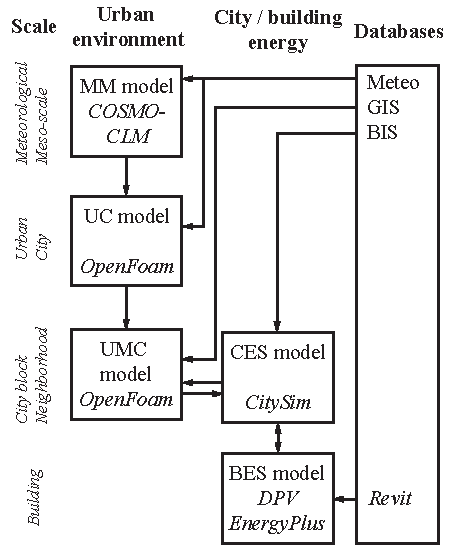
\includegraphics[scale=1.0]{figures/UMEM_overview_new}
\caption{EnergyPlus and CitySim coupling are part of the wider context. Each block in the diagram represents an environment, with the tool/engine name in italics (adapted from \citep{Dorer:2013vt})}
\label{fig:UMEM}
\end{figure}

This paper describes the achievement of several objectives:
\begin{enumerate}
  \item Automation of the process of simultaneous meta-data extraction from a building information model (BIM) for the creation of both building and urban-scale performance models for a real-world campus of buildings
  \item Co-simulate the urban and building scale models through concurrent information exchange
  \item Implement a simplified calibration procedure based on reconciling the co-simulation output results for a selected subset of buildings that have adequate measured energy performance data from the campus energy information system (EIS) 
\end{enumerate}

The first two objectives have been demonstrated in a simplified context in previous literature \citep{Thomas:2012wj}. The novelty of the current publication is an extension to this research through the modelling and co-simulation of a real-world case study campus. The third objective is completely novel in that no previous study has compared the results of a building and urban-scale co-simulation procedure to measured data from a real-world campus.

\subsection{Previous multiscale coupling studies}
Previous attempts of information exchange have been implemented between simulation engines at various scales. EnergyPlus and the TEP Urban Canopy Model program were coupled in order to quantify the influences of urban localized weather effects on whole building simulation \citep{Bueno:2011hi}. EnergyPlus has been coupled with ENVI-met, a micro-climate computational fluid dynamics (CFD) program
\citep{Yang:2012cr}.
% \subsection{Urban scale performance simulation}

\section{Methodology}
Some of the following methodology is developed in previous literature and is reiterated and explained in the context of a real-world implementation. The previous published research is clearly outlined at the beginning of each subsection.

\subsection{Coupling process}
The coupling process of a simplified single zone model and contextual surrounding buildings is outlined previously \citep{thomas2014multiscale,Thomas:2012wj}. This effort is based on the utilization of the Design Performance Viewer (DPV) and associated workflow. The DPV is a tool written to extract and simulate an EnergyPlus input data file (IDF) from an Autodesk\textsuperscript{TM} Revit\textsuperscript{TM} BIM \citep{Schlueter2009}. The main philosophy behind the tool is rapid simulation of the building information model from the earliest design possible and can be used throughout the life-cycle of the building including retrofit analysis \citep{Miller:2014tu}. This process is achieved by augmenting the information in the BIM with default values and abstracting information not relevant for energy simulation. The tool already has a simplified notion of surrounding buildings, which are modeled in the BIM as simple mass objects without further information and are exported as shading surfaces to EnergyPlus. This functionality is used for creating the CitySim mass scene and leads to a crude model of the urban context of the building. The existing DPV philosophy of allowing the designer to iterate rapidly on early design decisions based on feedback about the performance of the design remains. This approach includes streamlining the process where running a simulation requires no effort from the designer due to automatic creation of input files, execution and analysis of the results.

The coupling process of EnergyPlus and CitySim is shown in Figure \ref{fig:OverallWorkflowProcess}. First, the DPV is used to extract an EnergyPlus simulation model from the BIM. The DPV utilizes the Revit API to extract geometrical information about the building and the physical properties of walls, windows, doors, roofs and floors. This information is encoded in the BIM model as wall types, roof types,
floor types as well as window and door families. Wherever possible, the tool uses the layering and materials of the construction types, enhancing them with physical attributes relevant to EnergyPlus. Where not defined, it assumes default values.

\begin{figure}
\centering
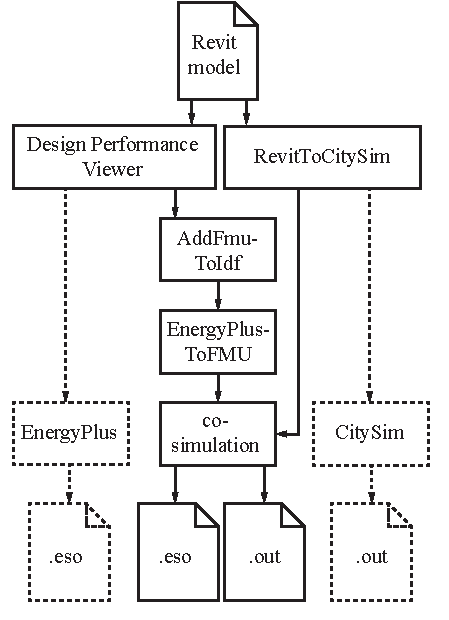
\includegraphics[scale=1.0]{figures/UMEM_Workflow}
\caption{Overview diagram of the coupling process including tools and outputs}
\label{fig:OverallWorkflowProcess}
\end{figure}

% \subsection{Geometry creation process}
Next, geometry is created to be used in both the CitySim and EnergyPlus models as buildings and surfaces surrounding the building targeted in the IDF. This feature of the DPV is used for including shading surfaces in the EnergyPlus simulation model: it uses so-called \emph{mass objects} in the BIM model as surrounding buildings. The DPV model views these buildings as a series of shading surfaces. A transformation is added on the DPV model that produces an input file for the CitySim solver. This file uses an XML format describing the buildings in a scene for simulation, including their construction types, geometry and systems for heating and cooling. The main BIM is extracted to the CitySim scene as one of the buildings to be simulated, with the properties of the construction types matching those in the DPV model. The glazing ratio is calculated based on the window and wall areas of the DPV model. Shading surfaces are grouped into buildings based on the mass object they were extracted from. These neighboring buildings use default construction properties for walls and roofs and we assign them a default glazing ratio. These defaults can be overridden by custom properties applied to the mass objects in the BIM much in the same way as the model elements of the main building are enriched with DPV information. 

As of version 8.1.0, EnergyPlus supports exporting a simulation model as a Functional Mock-up Unit (FMU) \citep{Nouidui:2014hq}. This feature introduces new IDF objects to specify the interface such an FMU exposes. These objects define which output variables are exported by the FMU and which variables are imported. The FMU export functionality is closely linked to the Energy Management System (EMS) of EnergyPlus. Co-simulation exchange variables either mimic an EnergyPlus schedule, an EMS variable or drive an EMS actuator. It was determined that in order to export an output variable using the FMU export functionality, the variable itself must also be output with an IDF object of type \emph{Output:Variable} or \emph{EnergyManagementSystem:OutputVariable} in the IDF file as well.

Since the model used by CitySim to simulate a building is more abstract than the model used by EnergyPlus, the EMS is used to aggregate certain values. CitySim does not model windows separately, so we calculate a weighted average of window and wall surface temperatures with EMS subroutines.

\begin{figure}
\centering
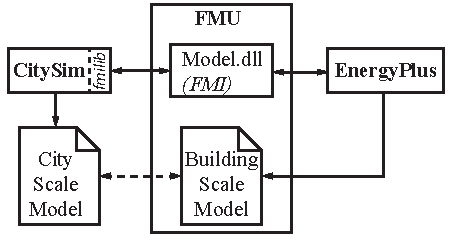
\includegraphics[scale=1.0]{figures/UMEM_FMU_Overview}
\caption{Simulation information exchange between CitySim and EnergyPlus using FMI}
\label{fig:FMUOverview}
\end{figure}

The process of augmenting the IDF file is automated with the EMS subroutines and FMU export objects. The script \emph{addfmutoidf.py}, written in the Python programming language, uses the \emph{parseidf} module to read in the IDF file and add the new IDF objects based on those found in the model.  This script reads in the list of surfaces defined in the IDF file and produces EMS scripts to aggregate and output the surface temperatures of the wall and the windows as well as any other output objects necessary.

The FMU creation process is the basis for coupling the two models at each timestep in the simulation. Figure \ref{fig:FMUOverview} illustrates this process from both the EnergyPlus and CitySim perspective. The augmented IDF file is fed to the \emph{EnergyPlusToFMI} script \citep{Nouidui:2014bo}. Once configured, this script produces an FMU file based on the augmented IDF file and the weather file to be used as well as a DLL file implementing the Functional Mock-up Interface that can load the IDF file, locate EnergyPlus and run the simulation. Table \ref{tab:FMUimports} and \ref{tab:FMUexports} outline the variables exchanged between EnergyPlus and CitySim through the FMI. We used the \emph{fmilib} library from the JModelica project to test the FMU produced \citep{Anonymous:ZZTfF80-}. We altered one of the sample programs (\emph{fmi\_import\_cs\_test.c}) to load the FMU, run it and print out the values exported from EnergyPlus. This code was then used as a guide to extending the CitySim solver to load FMUs for co-simulation.

On an hourly basis, CitySim performs a heating and cooling needs prediction step. The temperature determination step for the main building is replaced with the results of the EnergyPlus timestep as obtained through FMI library. The FMI library is used to send climatic and occupational data from CitySim to EnergyPlus (see Table \ref{tab:FMUimports}), and to receive data from EnergyPlus that are further used within CitySim for the next time steps (see Table \ref{tab:FMUexports}).

\begin{table}
\centering
\caption{Values imported by EnergyPlus from CitySim by the FMU}
\label{tab:FMUimports}
\centering
\begin{tabular}{|p{1.3cm}|p{1.9cm}|p{3.2cm}|}
  \hline
  \bf{Object (ep\_id)} &  \bf{Variable Name} & \bf{Description} \\
    \hline
Outdoor & Outdoor Drybulb & The outdoor dry-bulb temperature in $^{\circ}\mathrm{C}$ \\
     \hline
 & Outdoor Dewpoint & The outdoor dewpoint temperature in $^{\circ}\mathrm{C}$ \\
     \hline
 & Outdoor Relative Humidity & The outdoor relative humidity expressed in percent. \\
     \hline
 & Diffuse Solar & Diffuse horizontal irradiance in W/m$^2$ \\
     \hline
 & Direct Solar & Beam normal irradiance in W/m$^2$ \\
     \hline
 & Wind Speed & The outdoor wind speed in m/s \\
     \hline
 & Wind Direction & The wind direction in degrees (N=0, E=90, S=180, W=270) \\
     \hline
Zone & Occupation & Fraction of the maximum occupation (0.0-1.0) overrides the EnergyPlus occupation schedule with the CitySim stochastic schedule. \\
    \hline
\end{tabular}
\end{table}

\begin{table}
\caption{Values exported by EnergyPlus to CitySim by the FMU}
\label{tab:FMUexports}
\centering
\begin{tabular}{|p{1.3cm}|p{1.9cm}|p{3.2cm}|}
  \hline
  \bf{Object (ep\_id)} &  \bf{Variable Name} & \bf{Description} \\
    \hline
Wall, Roof & Outside Surface Temperature & The temperature on the outside of the surface in $^{\circ}\mathrm{C}$ \\    
    \hline
Wall & Average Outside Surface Temperature & The (weighted) average temperature of the surface on the outside in $^{\circ}\mathrm{C}$. This respects the temperatures of the windows on the wall, weighted by area. \\
    \hline
Zone & Total Heating Energy & The heating energy in Joules used in this timestep. \\
    \hline
 & Total Cooling Energy & The cooling energy in Joules used in this timestep. \\
    \hline
 & Zone Mean Air Temperature & The mean air temperature in the zone in $^{\circ}\mathrm{C}$ \\
    \hline
 & Ventilation Volume Flow Rate & The flow rate in $\mathrm{m}^3/\mathrm{s}$ (standard density) \\
    \hline
\end{tabular}
\end{table}

\subsection{Co-simulation simplified calibration}

{\color{red}This section will describe in detail the method for comparing the CitySim vs. EnergyPlus vs. Co-simulation and how we use the measured data as a comparison}

\section{Implementation}
\subsection{Campus case study}
{\color{red}This section will describe the ETH Hoenggerberg case study}

% \begin{figure}
% \centering
% 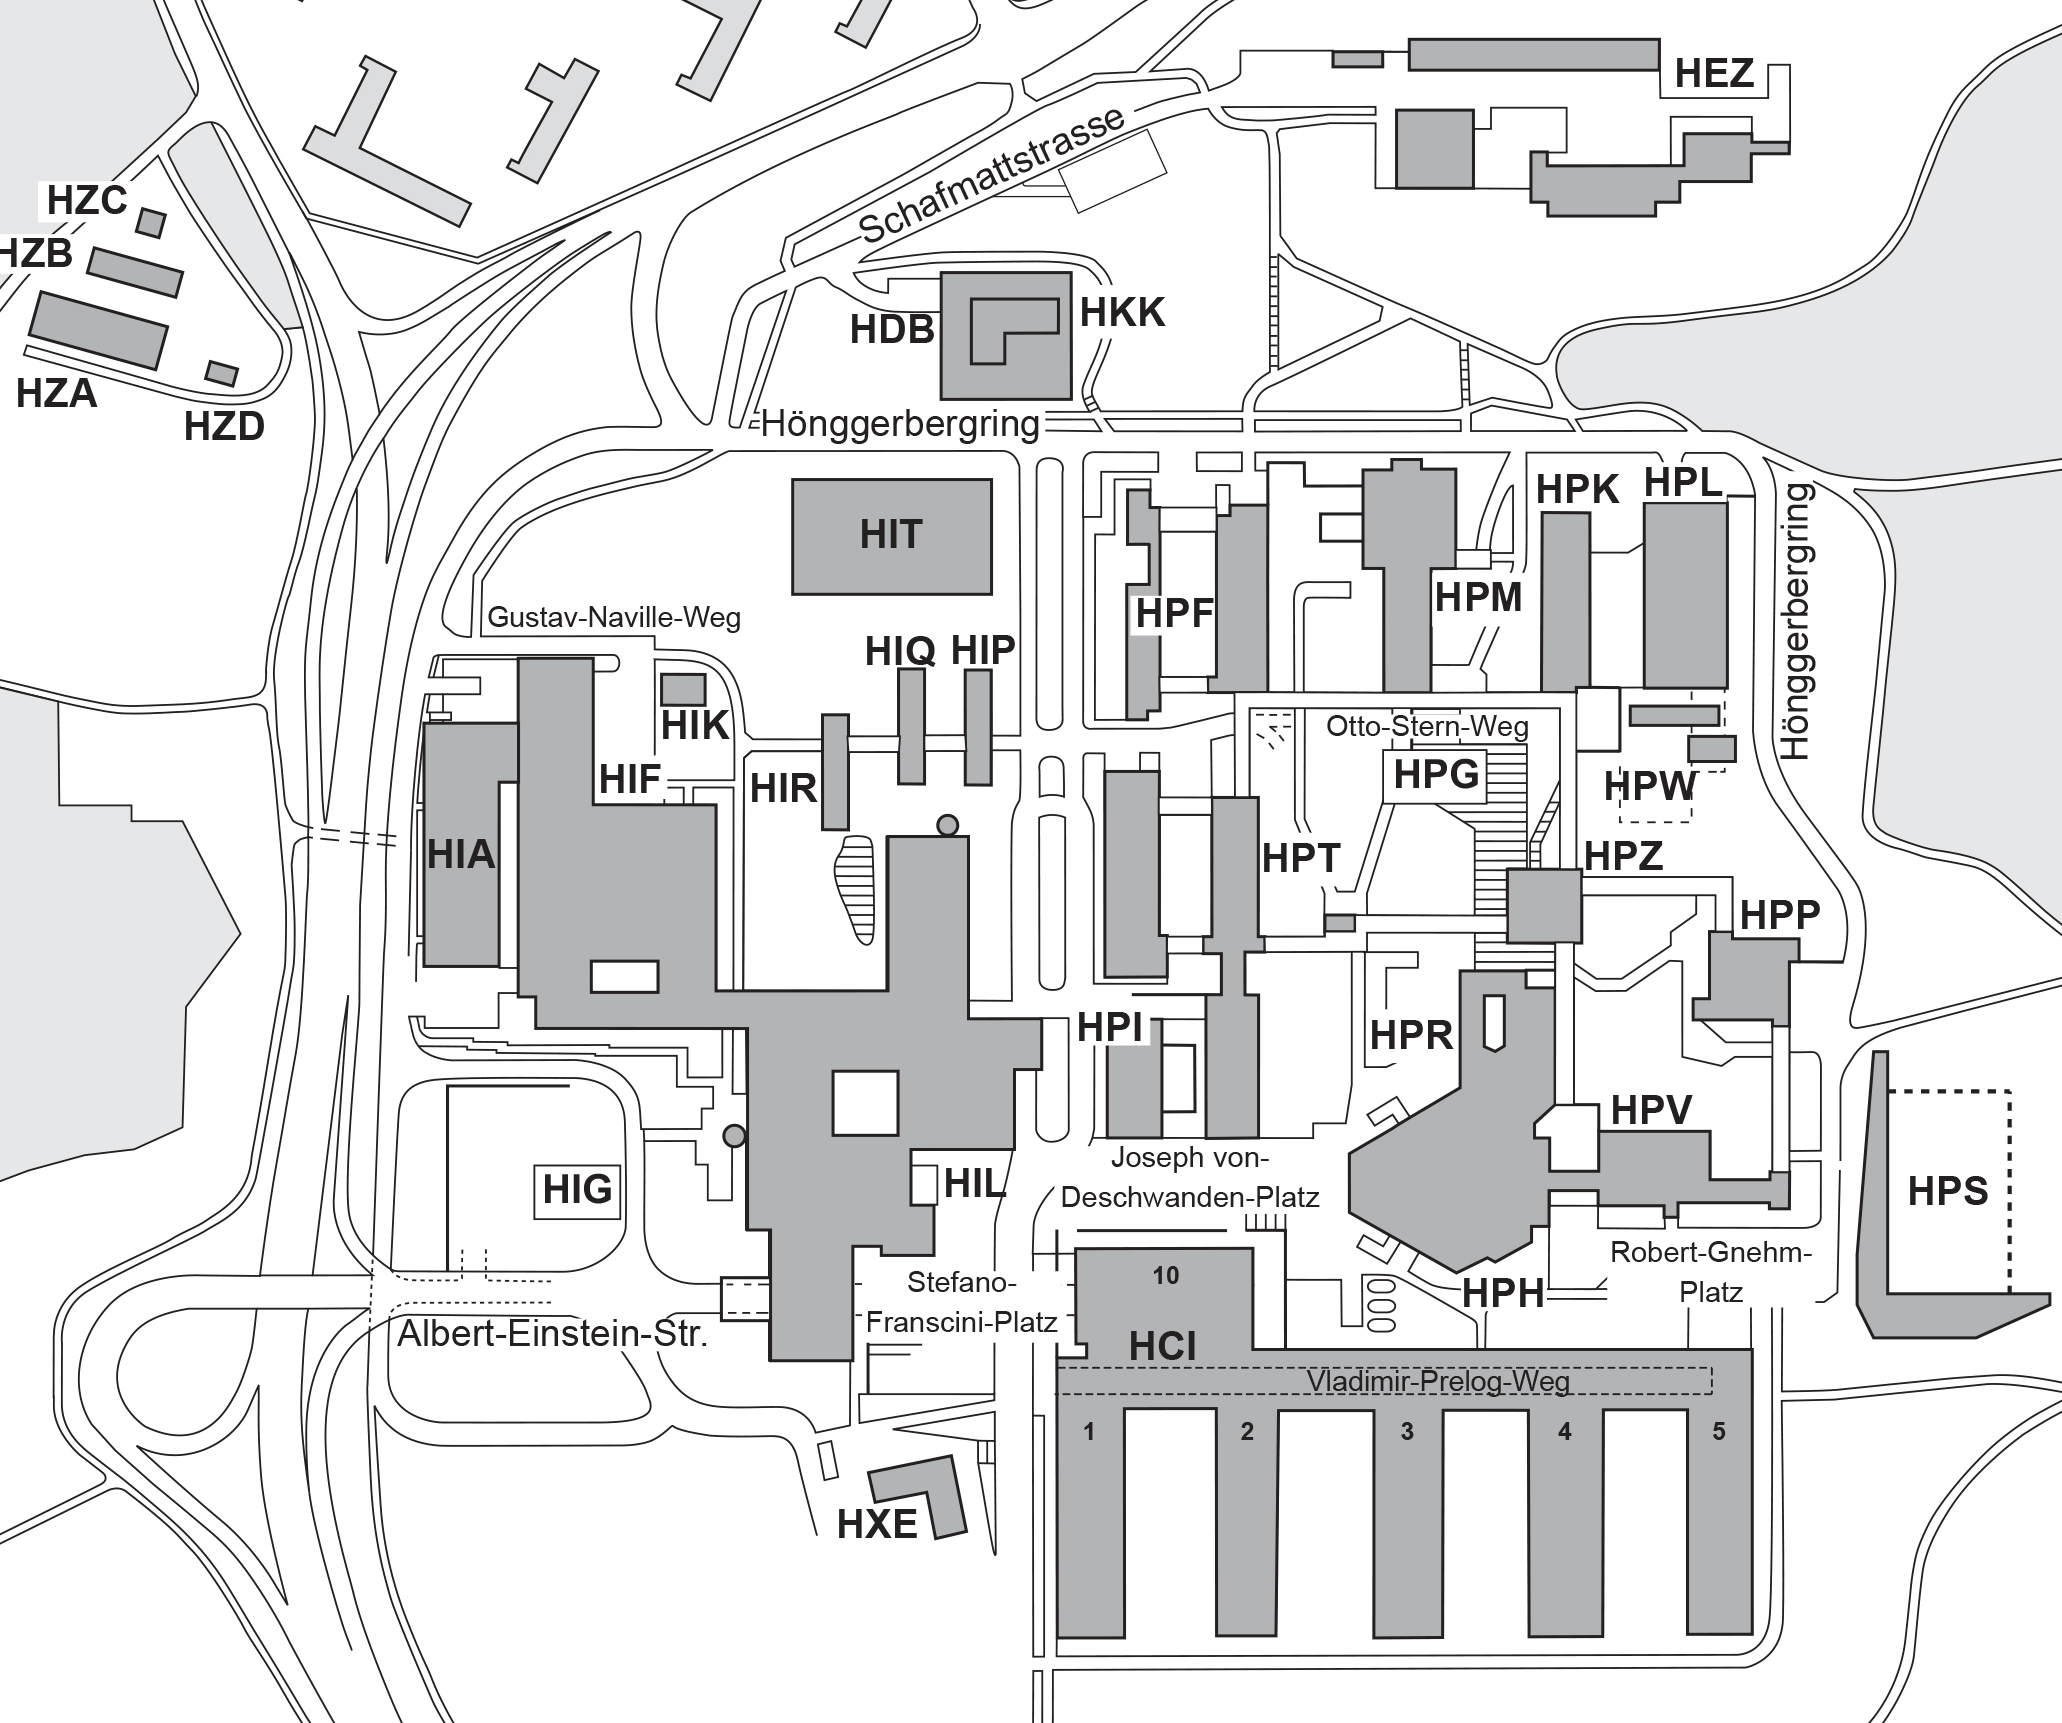
\includegraphics[scale=0.1]{figures/campusmap}
% \caption{Map of the case study campus}
% \label{fig:campusmap}
% \end{figure}

\subsection{Model development}
{\color{red}This section will describe the development of the Revit, CitySim and EnergyPlus models}
\begin{figure}
\centering
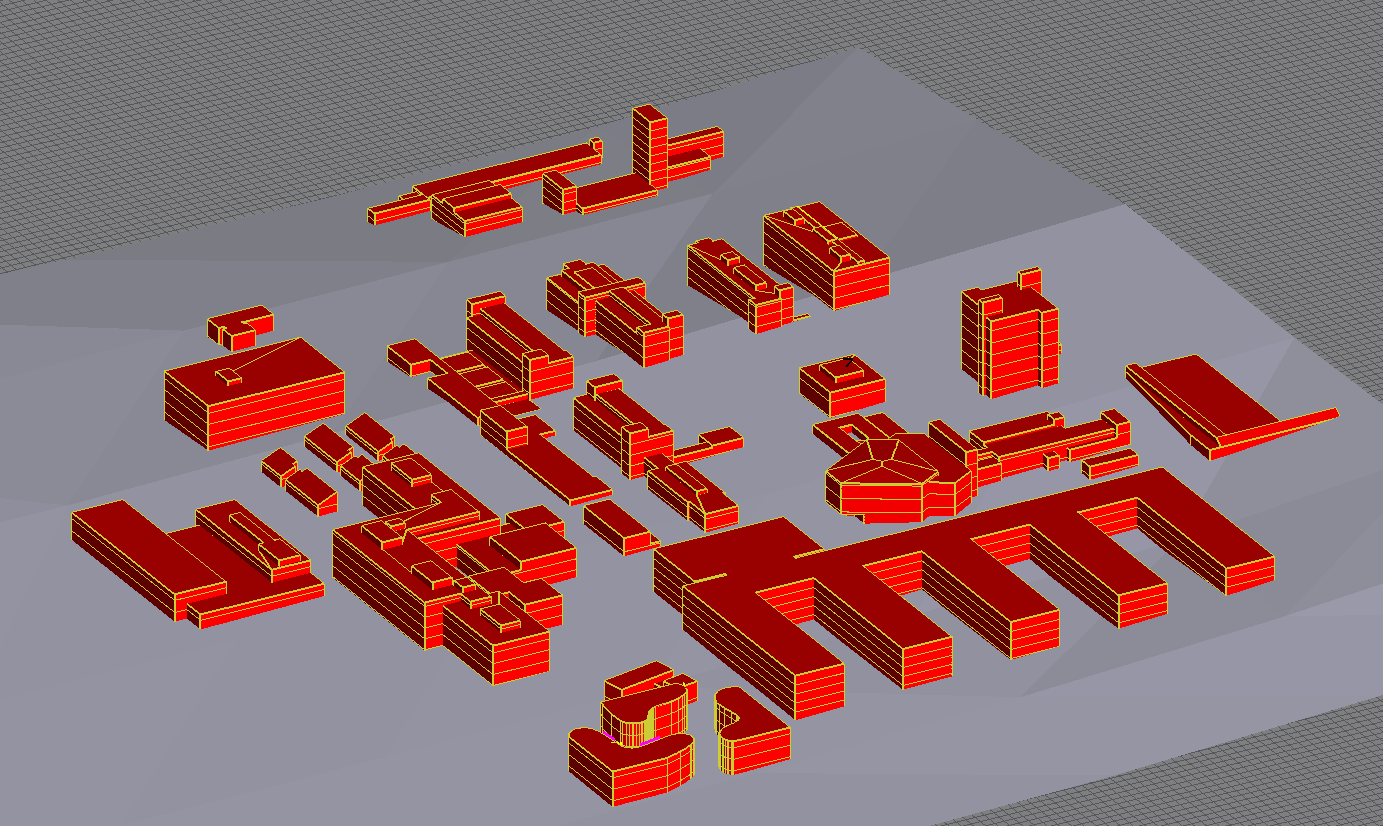
\includegraphics[scale=0.3]{figures/campuscitysim}
\caption{Campus modelled in CitySim}
\label{fig:campuscitysim}
\end{figure}

\subsection{Measured data collection and processing}

\begin{figure}
\centering
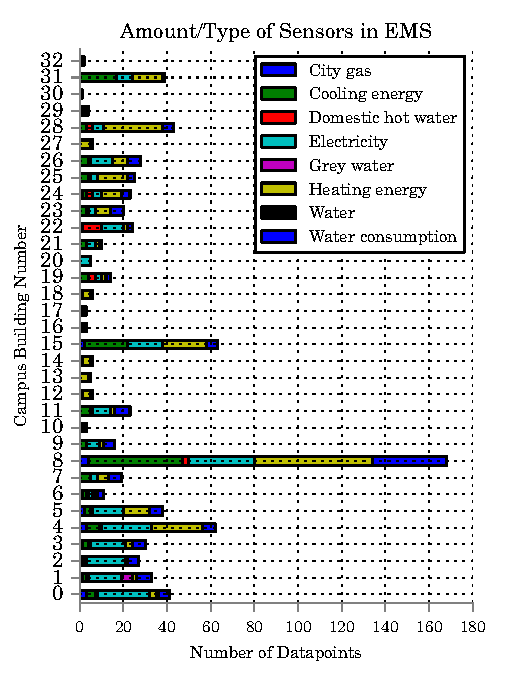
\includegraphics[scale=1.0]{figures/pointbreakdown_anon}
\caption{Available performance measurement points}
\label{fig:pointgraph}
\end{figure}

\section{Results}
{\color{red}Here we show all of the data of the comparison between the simulation outputs and the measured data from the campus}

\section{Discussion}


\section{Conclusion}

\subsection{Acknowledgements}


% The authors would like to acknowledge the ETH Z\"urich Campus Facilities Department.

\bibliographystyle{tBPS}
\bibliography{UMEM_CoSim}


\end{document}
